
\documentclass[sigplan,screen]{acmart}


%% Contributed by Gregor von Laszewski
\usepackage{textcomp}
\usepackage{hyperref}
%\usepackage[table]{xcolor}
% \usepackage[table]{xcolor}
\usepackage{colortbl}
\usepackage{MnSymbol}
%\usepackage{todonotes}
%\newcommand{\TODO}[1]{\todo[inline]{#1}}
%\newcommand{\NOTE}[1]{\textcolor{red}{[NOTE: #1]}}
%\newcommand{\FILE}[1]{\todo[inline,color=green!20]{File: #1}}

\newcommand{\GITHUB}[1]{\todo[inline,color=green!20]{
\href{https://github.com/laszewsk/mlcommons-uva/issues/#1}{GitHub Issue #1}}}


\setcopyright{none}
\settopmatter{printacmref=false}
\renewcommand\footnotetextcopyrightpermission[1]{}

%\usepackage{minted}
%\setminted{fontsize=\footnotesize,xleftmargin=1.5\parindent}

\usepackage{longtable}
\usepackage{fancyvrb}

% \usepackage{color}
% \usepackage{listings}
%\usepackage{xcolor}
%\usemintedstyle{trac}
%\definecolor{mblue}{rgb}{0.27,0.33,0.53}

\definecolor{friendlybg}{HTML}{f0f0f0}
\definecolor{lightgray}{rgb}{.9,.9,.9}
\definecolor{darkgray}{rgb}{.4,.4,.4}
\definecolor{purple}{rgb}{0.65, 0.12, 0.82}

% \lstdefinelanguage{bash}{
%   keywords={cms, cd},
%   keywordstyle=\color{blue}\bfseries,
%   keywords=[2]{set},
%   keywordstyle=[2]\color{green}\bfseries,
%   identifierstyle=\color{black},
%   sensitive=false,
%   comment=[l]{//},
%   morecomment=[s]{/*}{*/},
%   commentstyle=\color{purple}\ttfamily,
%   stringstyle=\color{red}\ttfamily,
%   morestring=[b]',
%   morestring=[b]"
% }

% \lstset{
%   language=bash,
%   extendedchars=true,
%   basicstyle=\footnotesize\ttfamily,
%   showstringspaces=false,
%   showspaces=false,
%   tabsize=2,
%   breaklines=true,
%   showtabs=false
% }



\newcommand{\REVISION}{8. Jul. 2023, revised 8 Dec. 2023}

\acmConference[MLCommons Science Working Group Report]{MLCommons Cloud Masking Benchmark with Early Stopage}{\REVISION}{}

%\acmBooktitle{Woodstock '18: ACM Symposium on Neural Gaze Detection,
%  June 03--05, 2018, Woodstock, NY} 
%\acmPrice{15.00}
%\acmISBN{978-1-4503-XXXX-X/18/06}

%%\acmSubmissionID{123-A56-BU3}

%%\citestyle{acmauthoryear}

\begin{document}



\newcommand{\TITLE}{MLCommons Cloud Masking Benchmark with Early Stopping}


\title[\TITLE]{MLCommons Cloud Masking Benchmark \\with Early Stopping \\ {\normalsize Version 1.0}}

\titlenote{\url{https://github.com/laszewski/papers/raw/master/vonLaszewski-cloudmask-nyu.pdf}}


\author{Varshitha Chennamsetti}
\affiliation{%
  \institution{New York University}
  \streetaddress{Center for Data Science\\
60 5th Ave}
  \city{New York}
  \state{NY}
  \postcode{10011}
  \country{USA}
}

\author{Gregor von Laszewski}
\email{laszewski@gmail.com}
\orcid{0000-0001-9558-179X}
\authornote{MLCommons authorized submitting author}
\affiliation{%
  \institution{University of Virginia}
  \streetaddress{Biocomplexity Institute\\
Town Center Four\\
994 Research Park Boulevard}
  \city{Charlottesville}
  \state{VA}
  \postcode{22911}
  \country{USA}
}

\author{Ruochen Gu}
\affiliation{%
  \institution{New York University}
  \streetaddress{Center for Data Science\\
60 5th Ave}
  \city{New York}
  \state{NY}
  \postcode{10011}
  \country{USA}
}

\author{Laiba Mehnaz}
\affiliation{%
  \institution{New York University}
  \streetaddress{Center for Data Science\\
60 5th Ave}
  \city{New York}
  \state{NY}
  \postcode{10011}
  \country{USA}
}



\author{Juri Papay}
\email{juri.papay@stfc.ac.uk}
\affiliation{%
  \institution{Rutherford Appleton Laboratory}
  \streetaddress{Harwell Campus}
  \city{Didcot}
  \postcode{OX11 0QX}
  \country{UK}
}

\author{Samuel Jackson}
\email{samuel.jackson@stfc.ac.uk}
\affiliation{%
  \institution{Rutherford Appleton Laboratory}
  \streetaddress{Harwell Campus}
  \city{Didcot}
  \postcode{OX11 0QX}
  \country{UK}
}


\author{Jeyan Thiyagalingam}
\email{t.jeyan@stfc.ac.uk}
\affiliation{%
  \institution{Rutherford Appleton Laboratory}
  \streetaddress{Harwell Campus}
  \city{Didcot}
  \postcode{OX11 0QX}
  \country{UK}
}

\author{Sergey V. Samsonau}
\affiliation{%
  \institution{New York University}
  \streetaddress{Center for Data Science\\
60 5th Ave}
  \city{New York}
  \state{NY}
  \postcode{10011}
  \country{USA}
}

\author{Geoffrey C. Fox}
\email{gcfexchange@gmail.com}
\affiliation{%
  \institution{University of Virginia}
  \streetaddress{Biocomplexity Institute\\
Town Center Four\\
994 Research Park Boulevard}
  \city{Charlottesville}
  \state{VA}
  \postcode{22911}
  \country{USA}
}

%%
%% By default, the full list of authors will be used in the page
%% headers. Often, this list is too long, and will overlap
%% other information printed in the page headers. This command allows
%% the author to define a more concise list
%% of authors' names for this purpose.
\renewcommand{\shortauthors}{Chennamsetti, von Laszewski, et al.}

%%
%% The abstract is a short summary of the work to be presented in the
%% article.
\begin{abstract}


In this paper, we report on work performed for the MLCommons Science Working Group on the cloud masking benchmark. MLCommons is a consortium that develops and maintains several scientific benchmarks that aim to benefit developments in AI. The benchmarks are conducted on the High Performance Computing (HPC) Clusters of New York University and University of Virginia, as well as a commodity desktop. We provide a description of the cloud masking benchmark, as well as a summary of our submission to MLCommons on the benchmark experiment we conducted. It includes a modification to the reference implementation of the cloud masking benchmark enabling early stopping. This benchmark is executed on the NYU HPC through a custom batch script that runs the various experiments through the batch queuing system while allowing for variation on the number of epochs trained. Our submission includes the modified code, a custom batch script to modify epochs, documentation\footnote{Disclaimer: the documentation from NYU no longer works due to a system upgrade at NYU. A transition to Singularity was recommended by the NYU system staff. This has been independently worked on by Ruochen Gu. However, as the accounts on Greene expired, this work could not be completed and was therefore not documented in this paper. For availability of portable code, please contact G. von Laszewski.}, and the benchmark results. We report the highest accuracy (scientific metric) and the average time taken (performance metric) for training and inference that was achieved on NYU HPC Greene. We also provide a comparison of the compute capabilities between different systems by running the benchmark for one epoch. Our submission can be found in a Globus repository that is accessible to MLCommons Science Working Group.



\end{abstract}

%%
%% The code below is generated by the tool at http://dl.acm.org/ccs.cfm.
%% Please copy and paste the code instead of the example below.
%%

\begin{CCSXML}
<ccs2012>
<concept>
<concept_id>10010405.10010432.10010437</concept_id>
<concept_desc>Applied computing~Earth and atmospheric sciences</concept_desc>
<concept_significance>500</concept_significance>
</concept>
<concept>
<concept_id>10010147.10010178.10010224.10010240.10010241</concept_id>
<concept_desc>Computing methodologies~Image representations</concept_desc>
<concept_significance>500</concept_significance>
</concept>
<concept>
<concept_id>10002951.10003317.10003359.10003360</concept_id>
<concept_desc>Information systems~Test collections</concept_desc>
<concept_significance>500</concept_significance>
</concept>
<concept>
<concept_id>10010583.10010737.10010749</concept_id>
<concept_desc>Hardware~Testing with distributed and parallel systems</concept_desc>
<concept_significance>500</concept_significance>
</concept>
</ccs2012>
\end{CCSXML}

\ccsdesc[500]{Applied computing~Earth and atmospheric sciences}
\ccsdesc[500]{Computing methodologies~Image representations}
\ccsdesc[500]{Information systems~Test collections}
\ccsdesc[500]{Hardware~Testing with distributed and parallel systems}



%%
%% Keywords. The author(s) should pick words that accurately describe
%% the work being presented. Separate the keywords with commas.
\keywords{cloud masking, cloudmesh, datasets, MLCommons, benchmark}


\received[Version from]{\REVISION}

\begin{comment}
\begin{center}
{\huge\bf \TITLE}
\end{center}

% \listoftodos

\tableofcontents
\listoffigures
\listoftables
\end{comment}

\clearpage

\settopmatter{printfolios=true}
\maketitle


\section{Introduction}


\nocite{las-2023-ai-workflow} % add to avoid running bibtex multiple times

Although artificial intelligence (AI) emerges as a powerful technology capable of transforming many aspects of life, several scientific niches/fields have yet to fully benefit from the advances in AI. Hence, there is a need for an initiative to increase awareness and push forward innovation in scientific fields where the potential for AI is huge but underexplored. 
MLCommons \cite{www-mlcommons-research}  is one such community effort that promotes AI for Science via benchmarking. MLCommons Science Working Group \cite{Thiyagalingam2022AIBF} has so far developed four scientific benchmarks in four varying fields: atmospheric sciences, solid-state physics, healthcare, and earthquake forecasting. In this paper, we present our submission to the cloud masking science benchmark in the atmospheric sciences domain. 

The objective of this benchmark \cite{Thiyagalingam2022AIBF} is to identify cloud pixels in satellite images (image segmentation). European Space Agency (ESA) \cite{www-sentinel92} has deployed a series of satellites to monitor the global environment. Amongst these satellites, Sentinel-3 has been made operational to focus on, among other missions, ocean surface topography and sea and land surface temperature (SST/LST). The process of the retrieval of SST and LST normally begins with cloud screening/masking, followed by the actual temperature estimation of the pixels that do not contain clouds. Cloud masking is performed since the presence of clouds can distort accurate estimations of temperature, making it a crucial step in the process of SST and LST estimation. 

Several methods have been used for this task ranging from rule-based \cite{Saunders1986AnAS,Saunders1988AnIM,Merchant2005ProbabilisticPB, Zhu2012ObjectbasedCA} to deep learning \cite{Li2019DeepLB,Domnich2021KappaMaskAC,Yan2018CloudAC,WIELAND2019111203,JEPPESEN2019247}. Some of the rule-based techniques have been threshold tests \cite{Saunders1986AnAS,Saunders1988AnIM} and Bayesian masking \cite{Merchant2005ProbabilisticPB}. Bayesian masking uses Bayes' theorem and prior meteorology information to generate probabilities for each pixel whether it contains cloud or not. Generalizing the process from a pixel, a cloud mask can then be generated from a satellite image. On the other hand, deep learning methods \cite{Li2019DeepLB,Domnich2021KappaMaskAC,Yan2018CloudAC,WIELAND2019111203,JEPPESEN2019247} use computer vision models and treat the cloud masking task as that of image segmentation. The most widely used model is U-Net \cite{Ronneberger2015UNetCN}, which is pretrained and designed for image segmentation, especially for large images.


In this paper, we document our submission to the MLCommons Science Working Group using a modified version of the cloud masking benchmark. We modified the reference implementation by introducing early stopping. As for data, we use a selected set of satellite images from Sentinel-3. We report the scientific metric (accuracy) and performance metric 
(scalability, training and inference time)
for this benchmark using NYU HPC Greene \cite{www-greene}. As part of this work, we have also done many in-depth experiments using UVA HPC Rivanna. These experiments are ran with the same hyperparameter settings as used in the reference implementation and were also used in this benchmark. However, the results for Rivanna are submitted separately together with a more  comprehensive analysis.

\section{MLCommons}

Scientific benchmarking is different from standard AI/ML benchmarking, particularly, their data differs in terms of both its volume and type \cite{las-2023-mlcommons-edu-eq}. The former requires heavy computing due to the I/O impact of its large-scale datasets, which leads to the use of supercomputers \cite{Farrell2021MLPerfHA}. MLCommons is a consortium that overlooks several scientific benchmarks in various scientific domains that can benefit from developments in AI. One of the working groups in MLCommons is the Science Working Group \cite{Thiyagalingam2022AIBF}, which maintains four different benchmarks at the time of writing this paper. A benchmark specifies a scientific task, provides the data for training and testing purposes, and defines a metric that needs to be reported by the contributors. In our case, the cloud masking reference benchmark provides 180GB worth of satellite image data. The scientific metric is the classification accuracy of pixels in satellite images being classified correctly, and the performance metric is the scalability over the number of GPUs (in our case one) and the time taken for training and inference. 
For each benchmark, a reference implementation is provided by the Science Working Group.

\section{Related Work}

From \cite{las-2023-cloudmask-related} we quote the general motivation and related research for cloud masking: ``Cloud masking is a crucial task that is well-motivated for meteorology and its applications in environmental and atmospheric sciences. Its goal is, given satellite images, to accurately generate cloud masks that identify each pixel in images as cloud or clear sky.

Since last century, several methods have been developed for cloud masking, ranging from rule-based techniques \cite{Saunders1986AnAS,Saunders1988AnIM,Merchant2005ProbabilisticPB, Zhu2012ObjectbasedCA} to modern deep learning approaches \cite{Li2019DeepLB,Domnich2021KappaMaskAC,Yan2018CloudAC,WIELAND2019111203,JEPPESEN2019247}. Among the more traditional, rule-based techniques, two popular methodologies have been threshold cloud screening \cite{Saunders1986AnAS,Saunders1988AnIM} and Bayesian cloud masking \cite{Merchant2005ProbabilisticPB}. 

Threshold screening methods consist of several threshold tests where spectral and spatial properties of satellite images are compared with those ranges that are believed to indicate the presence of a clear sky pixel. And those other pixels that are not labeled as clear sky are then flagged as cloudy. This school of methodologies was widely used from the late 1980s to the early 2000s \cite{Merchant2005ProbabilisticPB}. 

The gradual transition away from threshold screening methods was due to its long-criticized limitations: firstly, threshold settings rely heavily on domain expertise about indicators of cloudiness that may not be objective, which also makes later modification and updates difficult; secondly, thresholds provide users little flexibility in the trade-off between coverage and accuracy; third, threshold tests do not make use of all available prior information. These shortcomings of threshold screening methods are improved by later developed Bayesian methods \cite{Merchant2005ProbabilisticPB}.

The Bayesian approach applies Bayes' theorem on prior meteorology information to deduce for each pixel the probability of containing cloud or clear sky, and thereafter generating a cloud mask as output. As a result, these Bayesian approaches are fully probabilistic and make good use of prior information. Compared to threshold tests, Bayesian methods achieve better accuracy in predicting pixels' cloudiness, offering generality and conceptual clarity in its approach, and enhancing maintainability and adaptability largely \cite{Merchant2005ProbabilisticPB}. 

More recently, the rising popularity of deep learning has led to the use of CNNs for generating cloud masks. Deep learning methods \cite{Li2019DeepLB,Domnich2021KappaMaskAC,Yan2018CloudAC,WIELAND2019111203,JEPPESEN2019247} use computer vision models (CNNs) and treat the cloud masking task as that of image segmentation tasks. CNNs have achieved superior performance thanks to their automatic feature extraction ability. A research paper published in 2019 \cite{JEPPESEN2019247} introduces Remote Sensing Network (RS-Net), which is a CNN architecture branched out of U-Net \cite{RFB15a} for cloud masking and was shown to achieve higher performance compared to the state-of-the-art rule-based approach known as Fmask \cite{Zhu2012ObjectbasedCA}. KappaMask \cite{Domnich2021KappaMaskAC} and MSCFF \cite{Li2019DeepLB} are two additional U-Net based CNN model that outperformed Fmask. All these models have reported their performances on several satellite images such as Sentinel-2, Landsat, etc., and also made use of human-annotated (some assisted by software) ground truth values (See in Table \ref{tab:datasets}). On the other hand, MLCommons Cloud Masking Benchmark operates on SLSTR images from the newer Sentinel-3 satellite, which uses Bayesian approach generated cloud masks as ground truth. The reference implementation provided by MLCommons Science Working Group achieved 92\% classification accuracy on the Sentinel-3 test set \cite{Thiyagalingam2022AIBF}.

The aforementioned deep learning approaches towards cloud masking are by no means exhaustive. If you know about other significant cloud masking or deep learning approaches, please inform us and we will add them here.''

\begin{table*}[htb]
    \centering
    \caption{This table lists several methods used for cloud masking with their respective dataset, ground truth, and performance \cite{las-2023-cloudmask-related}.}
    \label{tab:datasets}
    \resizebox{1.8\columnwidth}{!}{
    \begin{tabular}{|l|c|l|l|l|l|}
    \hline
        {\bf} & {\bf Reference} & {\bf Dataset} & {\bf Ground-truth} & {\bf Model}  & {\bf Accuracy} \\ \hline
        1 & \cite{Merchant2005ProbabilisticPB} & ATSR-2 & Human annotation & Bayesian screening & 0.917\\ \hline
        2 & \cite{WIELAND2019111203} & Sentinel-2 & Software-assisted human annotation (QGIS) & U-Net & 0.90 \\ \hline
        3 & \cite{WIELAND2019111203} & Landsat TM & Software-assisted human annotation (QGIS) & U-Net & 0.89 \\ \hline
        4 & \cite{WIELAND2019111203} & Landsat ETM+ & Software-assisted human annotation (QGIS) & U-Net & 0.89 \\ \hline
        5 & \cite{WIELAND2019111203} & Landsat OLI & Software-assisted human annotation (QGIS) & U-Net & 0.91 \\ \hline
        6 & \cite{Li2019DeepLB} & GaoFen-1 & Human annotation & MFFSNet & 0.98, mIOU = 0.87 \\ \hline
        7 & \cite{Domnich2021KappaMaskAC} & Sentinel 2 & Software-assisted human annotation (CVAT) & KappaMask & 0.91 \\ \hline
        8 & \cite{JEPPESEN2019247} & Landsat 8 Biome and SPARCS & Human annotation & RS-Net & 0.956 \\ \hline
    \end{tabular}}

\end{table*}


\section{Dataset} 

The dataset used in our benchmark is described in \cite{las-2023-cloudmask-related} from which we quote: 
``MLCommons Cloud Masking Benchmark uses 180GB of satellite images from Sentinel-3 SLSTR (Level-1 processing, TOA Radiances and Brightness Temperature) satellite images. The dataset consists of 1070 images, captured during days and nights. The dataset also includes a cloud masking for each image, generated using Bayesian techniques. The reference implementation uses these cloud masks as ground truths for training and testing.

The dataset comes with the train-test split, where 970 images are used for training, and 100 images are used for testing. 
The images are of the dimension $1200 \times 1500$ with 15 different channels and 1 channel of Bayesian mask. Among the 15 channels, 3 channels are used to represent brightness, 6 channels are used to represent reflectance, and the remaining 6 channels are used to represent radiance. However, for the provided reference implementation, only a total of 10 channels, i.e., 6 channels of reflectance, 3 channels of brightness, and 1 channel of Bayesian mask are used as model inputs for training and testing.'' 

\begin{figure*}[htb]

\centering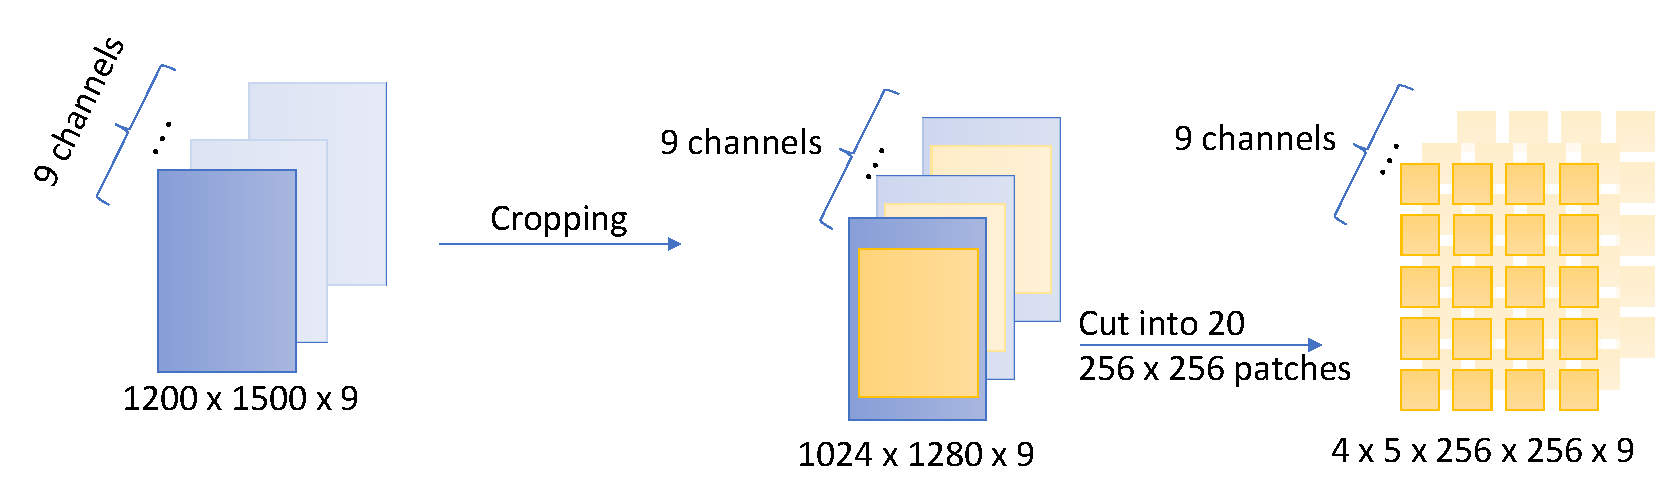
\includegraphics[width=0.75\textwidth]{images/cloudmask-preprocessing-training-data-2.pdf}
\caption{The preprocessing of the training data \cite{las-2023-cloudmask-related} .}
\label{fig:preprocessing-training}

\bigskip

\centering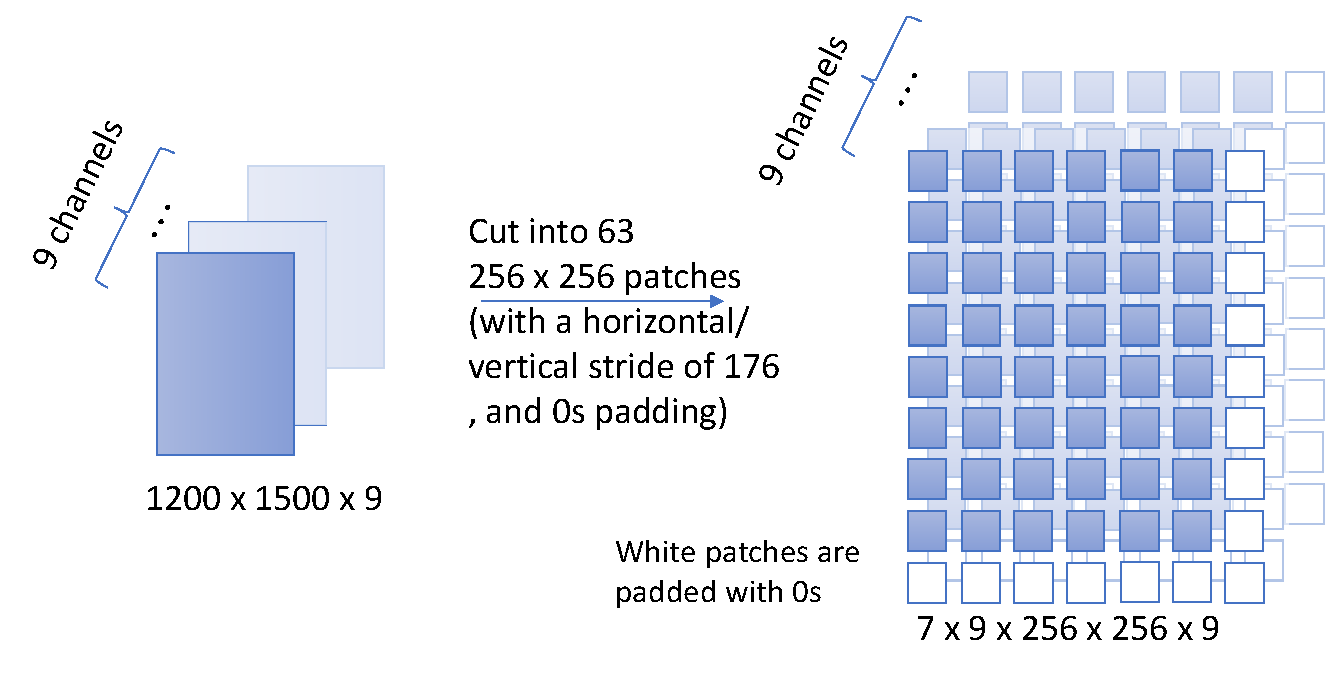
\includegraphics[width=0.75\textwidth]{images/cloudmask-preprocessing-testing-data-2.pdf}
\caption{The preprocessing of testing data \cite{las-2023-cloudmask-related}.}
\label{fig:preprocessing-testing}

\end{figure*}

\subsection{Data Loading and Preprocessing} \label{sec:preprocessing}

We quote from \cite{las-2023-cloudmask-related}:  ``For training data preprocessing, the images are first cropped from the dimension of $1200 \times 1500 \times 9$ to $1024 \times 1280 \times 9$ and then divided into 20 smaller-sized $256 \times 256 \times 9$ patches. After creating these patches out of each image in training set, we get a total of $19400$ patches for training. These patches are further split into training and validation set with $80/20$ split ratio, and then sent for training after shuffling. 

For the test dataset, the images are neither cropped nor shuffled. Instead, each test image are cut into 63 smaller patches of dimension $256 \times 256 \times 9$, by applying a horizontal and vertical stride of 176 pixels with zeros padding on the right and bottom edges of each image. We then get a total of $6300$ patches for entire test dataset. After getting the predictions from the model, these $256 \times 256 \times 1$ output patches (predicted cloud mask) are reconstructed to the size of $1200 \times 1500 \times 1$ and then evaluated with the Bayesian mask ground truth that has the same dimension. This preprocessing pipelines for training and testing are shown in Figure \ref{fig:preprocessing-training} and Figure \ref{fig:preprocessing-testing}.''

\subsection{Training}

We quote from \cite{las-2023-cloudmask-related} the training data processing methodology:
``During training, the model takes a preprocessed patch of dimension $256 \times 256 \times 9$, and generates a cloud mask of dimension $256 \times 256 \times 1$. Once the cloud masks have been generated by the model during training, the accuracy is reported as the percentage of total pixels that are correctly classified compared to ground truth'' \cite{las-2023-cloudmask-related}. 

\subsection{Testing}

We quote from \cite{las-2023-cloudmask-related} the testing data processing methodology:
``During testing, the model generates a cloud mask of dimension $256 \times 256 \times 1$ for each $256 \times 256 \times 9$ patch. For each pixel in the image, the model outputs the probability of that pixel containing clear sky. Pixels that have a probability higher than 50\% are labeled as clear sky, and cloudy otherwise. Then, those patches are then reconstructed back to full-size masks of dimension $1200 \times 1500 \times 1$.'' 

The geographic locations of the images used in the testing can be found in \cite{las-2023-cloudmask-related}.



\section{Model}

The MLCommons Cloud Masking Benchmark \cite{Thiyagalingam2022AIBF} reference implementation uses a U-Net \cite{Ronneberger2015UNetCN} model. The architecture of U-Net is such that the model can output a label for each pixel in the image, instead of one label for the image. For this reason, the model first creates a contracting path to get deeper context and then has a symmetric expanding path to increase resolution that promotes localization of outputting a label.

\section{Logging}

Logging is an important tool for reproducing experiments and results. MLCommons uses a standard logging library called MLCommons MLPerf/MLlog \cite{github-mlcommons-logging} to produce logs that contain information about each run. This is done so that the benchmark submission can pass through logging checker to be accepted by MLCommons. MLlog records standard events such as "INTERVAL START", "INTERVAL END" and "POINT IN TIME" with key-value pairs. Hence, the logs generated from our experiments are one of the many artifacts submitted to MLCommons. 
However, the MLlog records are not easily human readable. This is especially important during the modification and debugging of new reference implementations. For that reason, the UVA team uses log generated by  cloudmesh StopWatch  (which is part of cloudmesh-common) \citep{cloudmesh-stopwatch}, which provides multiple output formats including a human-readable summary table and explicitly named timers and events.  Furthermore, cloudmesh StopWatch has an extension that automatically creates MLlog entries, which saves the effort to augment the code explicitly for MLlogs . Furthermore, postprocessing the log data is far easier using cloudmesh StopWatch. Although this library was used extensively by the UVA team leading to easy-to-understand human readable logs, the NYU team elected to not utilize it requiring to run always a custom log parser instead of just looking into the log files for the results, making the overall inspection and modification of the code during the development more time consuming.

\section{Experiments}
\label{sec:exp}

In this section, we describe our submissions of the cloud masking benchmark to the MLCommons Science Working Group. First, we describe the compute resources we used for the benchmark in Section \ref{sec:hw}. Then, we go through the details of the benchmark outlining the code modifications in Section \ref{sec:code}, The installation in Section \ref{sec:install}, and how to produce the results in Section \ref{sec:parallel}.

\subsection{Compute Infrastructure}
\label{sec:hw}

This study was conducted on different compute infrastructures. These include: a commodity desktop, the HPC at UVA called {\em Rivanna}, and the HPC at NYU called {\em Greene}. We describe the computing resources in more detail and summarize some of their characteristics in Table \ref{tab:hwoverview}\footnote{The table represents the status of the machines in July 2023, it may have changed since then, but the studies are done with these resources.}.


\begin{table*}[htb]
    \caption{Overview of the computing resources used \cite{las23-cloudmask}, at the time of writing this paper.}
    \label{tab:hwoverview}
    \begin{center}
    \begin{tabular}{|l|r|r|r|r|r|r|r|}
        \hline
            {\bf Machine}  & {\bf Cores} & {\bf Memory} & {\bf GPU}   &   {\bf Memory} & {\bf GPUs} & {\bf Nodes}  & {\bf Commissioned} \\ 
                     &  {\bf /Node} & {\bf /Node}  &  {\bf Type}  & {\bf /GPU}     &   {\bf /Node}        & & \\
        \hline
        \hline
        Rivanna (UV)    & 128 & 2000GB   & A100 & 80GB &  8  & 10 & Feb 2022 \\
                        & 128 & 1000GB   & A100 & 40GB &  8  &  2 & Jun 2022 \\   
                        & 28  & 255GB    & K80  & 11GB &  8  &  8 & Jun 2018 \\
                        & 28  & 255GB    & P100 & 12GB &  4  &  4 & Jan 2018 \\
                        & 28  & 188GB    & V100 & 16GB &  4  &  1 & Feb 2019 \\
                        & 40  & 384GB    & V100 & 32GB &  4  & 12 & Feb 2021 \\
                        & 36  & 384GB    & V100 & 32GB &  4  &  2 & Apr 2022 \\
                        &  64 & 128GB     & RTX3090   & 24GB    & 4   &  5 & Feb 2023         \\
                        & 40  & 384GB    & RTX2080TI & 11GB & 10  &  2 & May 2021 \\
         \hline
         Greene (NYU)	& 48	& 384	& RTX8000 	& 48	& 4	& 73 & Nov 2020\\
	        & 48	& 384	& V100 	    & 32	& 4	& 10 & other dates \\
	        & 40	& 512	& V100 	    & 3     & 8 & 1  & not published \\
	        & 40	& 384	& V100 	    & 32    & 4	& 1  & \\
	        & 40	& 384	& V100 	    & 16    & 4	& 6  & \\
	        & 80	& 1024	& A100  8358	& 80    & 4 & 31 & \\
	        & 64	& 512	& A100  8380	& 80    & 4 & 9  & \\
%	        & 96	& 512	& MI50              & 32    & 8 & 20 & \\
%	        & 128	& 512	& MI100	            & 32    & 8 & 3  & \\
%	        & 128	& 512	& MI250	            & 64    & 8 & 2  & \\

         \hline
         Desktop 5950X     &  32 & 128GB     & RTX3090   & 24GB    & 1 & 1 & Feb 2022   \\
         \hline
    \end{tabular}
    \end{center}

\end{table*}

\paragraph{NYU Greene HPC} NYU Greene is a general-purpose cluster at New York University that supports a variety of job types and sizes. This includes jobs requiring multiple CPU cores, multiple GPU cards, or terabytes of memory. For this submission, we use V100 GPUs and RTX8000. More specifications of the cluster can be found on the NYU HPC Greene homepage \cite{www-greene}.

\paragraph{UVA Rivanna HPC} UVA Rivanna is a cluster built on a condominium model where different groups add resources to the cluster to then be shared with its entire user base. As such the cluster is frequently updated and has due to its evolving updates a variety of GPUs. The various GPUs and their placement on the servers are listed in Table~\ref{tab:hwoverview}.

\paragraph{AMD 5090X RTX3090 Desktop} The desktop is a commodity custom built desktop with fast NVMe and an RTX connected to PCIe4 with more details listed in Table~\ref{tab:hwoverview}. As the RTX3090 is built using the Ampere architecture from NVIDIA it performs similarly to an A100 when memory is not an issue. When using 32-bit it will be even faster. However, we have not utilized this for this application.


\subsection{Code modifications}
\label{sec:code}

The benchmark's reference implementation was provided by Rutherford Appleton Laboratory (RAL) \cite{Thiyagalingam2022AIBF,github-laszewsk-mlcommons}. 
Additional timers were added by UVA and RAL and were available since July 2022 with minor updates since then. 
The original accuracy calculation used as accuracy a threshold that was only based on booleans if pixels were a cloud or not rather than a continuous numerical value. This had as a consequence that no significant changes in accuracy could be observed in different experiments. For this reason, a numerical accuracy value was introduced by the RAL team in early Dec 2022. 
UVA developed, for their version, the ability to customize the analysis of the runs through a portable Jupyter notebook that takes as input the FAIR \cite{www-fair} data produced by running the code via the convenient and easy-to-use cloudmesh experiment executor \cite{github-cloudmesh-ee,las-2023-escience-cloudmask,las-2023-ai-workflow}. This setup allowed for smooth hyperparameter experimenting that goes beyond just modifying the number of epochs as with the NYU code and instead allows easily a hyperparameter grid search. However, for this study, we restricted the test of parameters to just the number of epochs to align our experiments with NYU's.

\paragraph{Modification of the code at NYU} 
The NYU team reported that the accuracy value does not change while increasing the number of epochs to the UVA and RAL teams. This led the RAL and UVA team to release an updated version as described previously in early Dec. 2022 \cite{www-mlcommons-science-github}. This version was used as the basis for the NYU benchmarks.
The NYU team added to their modified version the ability to use early stopping \cite{Caruana2000OverfittingIN} to try to explore and avoid overfitting. The code was augmented with additional random seed initialization for Python random, TensorFlow, and NumPy. A batch script was developed that allows to run multiple epoch values through the queuing system. This allowed us to run more than one experiment and report the variance in the performance with more confidence. However, it only allows the use of one hyperparameter setting for all epoch runs.


\subsection{Installation}
\label{sec:install}

\paragraph{Installation on UVA Rivanna} UVA created an updated installation instruction that is the basis for porting to other machines and was successfully used by NYU. Although the UVA code was first deployed using bare metal software, the UVA team changed it to use Singularity in order to stay up to date with NVIDIA's most recent software releases that are deployed via the containers as recommended by NVIDIA. This change makes overall deployment easier. In principal, this deployment can be replicated on any machine that supports container frameworks such as Singularity.

\paragraph{Installation on NYU HPC Greene} The NYU team provided, for NYU Greene, specific updates to the installation documentation using bare metal deployment. This includes nuances of system-specific features of Greene that were available before July 2023. The NYU team, with the help from UVA, worked on installing and running the original reference implementation provided by MLCommons on HPC Greene in bare metal.  This was done to make sure the reference implementation can be successfully run on NYU Greene before the code was modified. 
The documentation included modifications to use specific Greene system staff provided modules for Python and TensorFlow.  
Although Greene supports Singularity, the NYU team decided (in contrast to UVA) to continue to use the bare metal deployment. Unfortunately, as of July 2023, this deployment could no longer be replicated as the underlying NVIDIA CUDA libraries on Greene were updated and the bare metal versions used were no longer supported by the systems staff. As a result, the Greene documentation and code are no longer kept up-to-date.
In an independent work conducted by Ruochen Gu, a version for Greene was developed that uses Singularity with overlays. However, as accounts on Greene expired, this code is also no longer maintained but could be used by Greene users with appropriate updates.


\paragraph{Portability} Groups that would like to port it to other machines may get inspired either by the bare metal deployment instructions or by the UVA Singularity deployment using images directly distributed by NVIDIA for TensorFlow \cite{las-2023-escience-cloudmask}. The code from UVA does not use overlays but is more sophisticated and easier to use while using cloudmesh-ee which allows hyperparameter searches by leveraging batch and non-batch compute resources.

\paragraph{Reproducibility} The code developed by UVA and especially the use of the cloudmesh-ee (experiment executor) \cite{github-cloudmesh-ee,las-2023-escience-cloudmask} allows for sophisticated result logging promoting the FAIR principle.

\subsection{Parallelization}
\label{sec:parallel}

\paragraph{Parallelization at NYU Greene} The experiments were run on NYU HPC Greene for each experiment in embarrassingly parallel fashion by leveraging the queuing system's capability of running jobs concurrently.
The NYU team reused the cloudmesh YAML configuration contributed by the UVA and RAL team 
that uses YAML files to initialize the hyperparameters for its experiments.
The NYU team integrated this logic into a custom SLURM script to generate such YAML files 
customarily, such that one file was sufficient to run all the given jobs in parallel, without having to run these jobs separately. Upon suggestion from UVA the NYU team also added the functionality for saving different models in different directories while the jobs are running in parallel given the same hyperparameter setup, such that no model overwriting can take place. As multiple jobs are executed from the same directory, careful management of filenames is integrated in the code. The jobs submitted to SLURM are managed as job arrays.

\paragraph{Parallelization at UVA Rivanna} Using the cloudmesh experiment executor (cloudmesh-ee) the UVA team can conduct easily hyperparameter grid searches as well as execute them in a coordinated fashion on multiple supercomputers simultaneously \cite{las-2023-ai-workflow,github-cloudmesh-ee,las-2023-mlcommons-edu-eq}. Cloudmesh-ee creates easily reproducible runs and results following the FAIR principle. The usability of this tool has previously been shown also for other scientific applications. The software has been successfully utilized to manage long-running hyperparameter searches for the MLCommons earthquake forecasting. As this tool and its configuration files take care of utilizing separate directories for running the code and producing the output, no modification to the original code was needed other than switching to the updated YAML configuration files. In contrast to the NYU implementation, cloudmesh-ee enables the user to specify ranges for all hyperparameters in a single YAML configuration file. A single command line is used on the YAML file to generate an extensive hyperparameter search without modification of the program. Thus, instead of spending a significant amount of time generating various YAML files (as is the case for the NYU implementation), this is accomplished in seconds through cloudmesh-ee for all hyperparameters and not just a single one (e.g. epoch).

Cloudmesh experiment executor is based on an easy-to-use but sophisticated enhancement to batch queuing script management that we can apply to SSH, SLURM~\cite{www-slurm}, and LSF~\cite{www-lsf}. To control the permutations, a simple configuration parameter file is specified in YAML format~\cite{github-cloudmesh-ee} and can be started in a one-line command. 
When executing, it creates for each experiment a unique directory, in which the code and configuration parameters are stored. This allows the reproduction of a single experiment from within this folder given a unique set of configuration parameters. When the experiment is executed, all output files are stored in the directory. Thus, it promotes the implementation of the FAIR principle, as input and output files are available.
This provides a more integrated and more flexible approach than traditional shell scripts.
Furthermore, each experiment is submitted as its own job and thus projects smaller tasks that fit better in the boundaries of the queuing system policies we encountered. Submission in parallel has the advantage that the overall wait time in the queue is reduced as at UVA it takes longer to obtain more resources with time-consuming requests. Lastly, we evaluated the usability of cloudmesh-ee with an undergraduate. It was possible for the student not familiar with the cloud masking benchmark to run the benchmark within one day \cite{las-2023-escience-cloudmask} using cloudmesh-ee.

The reasons why the UVA team chose cloudmesh-ee is not only because it was available before this effort started, but because of additional reasons listed in Table~\ref{tab:advantage-ee}, where green highlighted areas show which system has a perceived advantage and white fields show no advantage. At NYU the educational experience of recreating a small portion of the cloudmesh-ee framework stood in the foreground, hence the team did not use cloudmesh-ee and instead developed an alternative, yet more  limited approach.
In addition, we can leverage the cloudmesh compute coordination framework (cloudmesh-cc) that can submit the hyperparameter searches onto a heterogeneous set of HPC machines in parallel \cite{las-2023-ai-workflow,github-cloudmesh-cc,las22-cloudmesh-cc-reu}. The tool creates first a workflow for executing all hyperparameter experiments.


\newcommand{\OK}{\cellcolor{green!10}}
\newcommand{\GR}{\cellcolor{gray!10}}

\begin{table}[p]

\caption{Comparison between the two approaches to run the benchmark. NYU chose to use a batch script based approach, while UVA used cloudmesh-ee}\label{tab:advantage-ee}

\centering
{\fontsize{8pt}{8pt}\selectfont
\begin{tabular}{|p{0.3\columnwidth}||p{0.3\columnwidth}|p{0.3\columnwidth}|}
    \hline
     \rowcolor{gray!10}{\bf Comparison}             & {\bf Batch script} &  {\bf cloudmesh-ee} \\
     \hline
     \hline
     \GR Installation & \OK Easy as distributed with code as bash script & \OK Easy as distributed with code through pip install\\
     \hline
     \GR Submission & \OK sh script with loop & \OK sh script that contains every job to be submitted \\
     \hline
     \GR Queuing System & SLURM & \OK SLURM, LSF, ssh \\
     \hline
     \GR Uses SLURM Job Arrays & Yes. However in case of resubmission of some jobs, job arrays are more complex then needed & Not by default but could be added. Instead Jobs can be managed on mass through scripts, which is equivalent in this case. \\
     \hline
     \GR File Management  & Files and directories are hard-coded and are not visible in the YAML file without inspecting the code & \OK Directories and files are created relative to the script execution directory thus allowing FAIR. Their names are automatically derived from the combination of hyperparameters specified  \\
     \hline
     \GR Program copy & A program copy is not generated & \OK For each experiment its own program copy is generated manifesting the FAIR principle as the program becomes part of the metadata \\
     \hline
     \GR Parameter specification & For each experiment its own YAML file needs to be generated by hand to modify other hyperparameters than epochs & \OK A single YAML file can be used to create many experiments allowing a hyperparameter grid search\\
     \hline
     \GR Direct parameter search & only epochs & \OK all parameters incl. epoch are supported\\
     \hline
     \GR Experiments can be repeated easily without overwriting old results & No & \OK yes \\
     \hline
     \GR Experiments form different computers can easily be merged & No & \OK Yes \\
     \hline
     \GR Single experiments can easily be rerun in case of failure & No & \OK Yes \\
     \hline
     \GR Logging & Based on MLPerf logging and is not easily human readable & \OK Based on MLPerf Logging but is automatically created from named timers and events \\ 
     \hline
    \GR Has been used for other MLCommons applications & No & \OK Yes \\
    \hline
    \GR Was previously available and is not new development & No & \OK Yes \\
    \hline
    \GR Learning curve & High as file management difficult to understand for graduate and undergraduates, and due to the need to create for each adjustable parameter its on YAML file & \OK Easy, proven to be usable for an undergraduate in less then an hour, due to only one YAML file needed for all experiments and the separation of the runtime environment for each experiment. \\
    \hline
    %\GR Perceived value in $\star$s  & $\star\star$ & \OK $\star\star\star\star\star\star\star\star\star\star\star\star$ \\
    %\hline
\end{tabular}
}

\end{table}

\subsection{Results} 

Using two different HPC systems, we now report selected performance (time per epoch) and scientific metrics (accuracy) results, while focusing mostly on data generated on NYU Greene.

\paragraph{Results from NYU Greene} The NYU team trained the model for a total of 200 epochs with early stopping \cite{Caruana2000OverfittingIN} and a patience of 25 epochs. We chose 25 epochs as the patience since the loss curve for the validation set exhibits considerable fluctuation as shown in Figure \ref{fig:Validation loss}. The fluctuation on the training accuracy curve as well as the difficulty of training this model is suspected to be caused by the usage of Bayesian masks as the ground truth \cite{Thiyagalingam2022AIBF}. We use a learning rate of $1e-3$ with a batch size of $32$. The remaining hyperparameters such as the crop size, patch size, train test split, etc., are kept the same as those from the reference implementation. We ran each of our experiments $5$ times and report the average accuracy and training/inference times.


Table \ref{tab: Results} shows the results of our best model on both V100 and RTX8000 GPUs. Figure \ref{fig:Training loss} shows the training loss for the five runs on the same seed, and we see that run 2 performs the best with the least loss. We observed for this benchmark the best model weights at epoch 147, and an accuracy of 0.896 while using early stopping. The train and validation loss curve for run 2 is shown in Figure \ref{fig:Losses of Run 2}. The average inference accuracy achieved in 5 runs is 0.889.

\paragraph{Comparative Results from UVA} While the results from NYU have been created using a shell script, the results from UVA have been created with the convenient cloudmesh-ee \cite{las-2023-ai-workflow,github-cloudmesh-ee}. We used cloudmesh-ee to create all results on UVA's Rivanna HPC. We added results obtained from NYU's Greene and show the comparative time consumption for a run with one epoch in Figure \ref{fig:epoch-compare}. We observe that the fastest machines are an NVIDIA station using the built-in raid followed by a custom build desktop with fast NVMe. 
The second fastest machine is a custom-designed desktop with an RTX3090 and fast NVMe storage.
The third fastest machine is an NVIDIA DGX node that is built into Rivanna while using the local NVMe storage. 
Both Rivanna and Greene utilize a shared file storage system that slows down the capabilities of the GPU cards while not being able to keep up with the calculations. This is shown in Figure \ref{fig:epoch-compare} as all machines using non-local storage perform significantly slower.
The Rivanna K80 performs the worst in our comparison due to its older hardware.
We also observed a large amount of variations as the server may be used in multi-user mode (indicated by the black lines). To guarantee no disturbance by others it is recommended to use exclusive server nodes. However, variations to access data on the shared file system can not be isolated.


\paragraph{Availability} The results are publicly available at \cite{www-mlcommons-cloudmask-results}.


\begin{figure}[htb]
\centering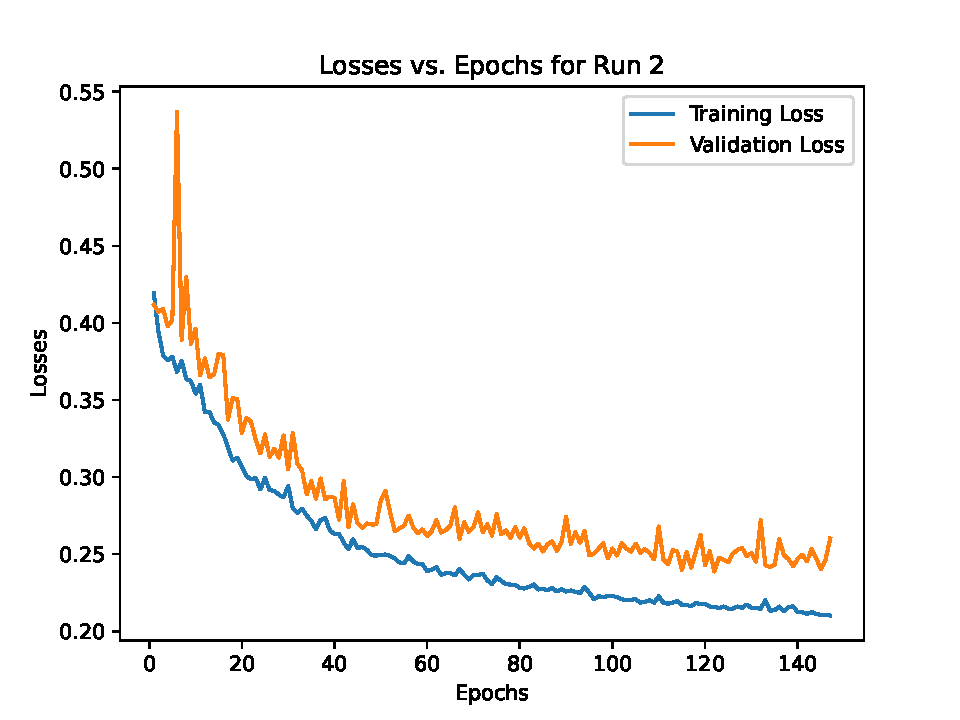
\includegraphics[width=1.0\columnwidth]{images/epoch_vs_loss-2.pdf}
\caption{Training and Validation Loss of Run 2 on NYU Greene.}
\label{fig:Losses of Run 2}
\end{figure}

%This model is run on xyx gpu. We need to add the best model for the other GPU as well, experiments yet to be run.


\begin{table*}[thb]
    \centering
    \caption{This table shows the results. Here the time for training and inference is reported as the avg. time per epoch for both training and inference.}
    \begin{tabular}{|l|l|l|l|l|l|l|l|}
    \hline
        Epochs & Seed & Train acc. & Test acc.  & avg. train time  & avg. inference time & GPU & Machine\\ \hline
        200 & 1234 & 0.895950 & 0.884168 & 142.47 & 1.73 & v100 & Greene \\ \hline
        147 & 1234 & 0.908647 & 0.896051 & 98.75 & 1.46 & v100 & Greene\\ \hline
        162 & 1234 & 0.897208 & 0.890086 & 108.16 & 1.44 & v100 & Greene\\ \hline
        200 & 1234 & 0.897057 & 0.889887 & 126.44 & 1.53 & v100 & Greene\\ \hline
        183 & 1234 & 0.896541 & 0.885192 & 121.21 & 1.41 & v100 & Greene \\ \hline
    \end{tabular}
    \label{tab: Results}
\end{table*}

%Still need to add results from Rivanna, and the desktop if Professor Gregor has run that.

\begin{figure}[htb]
\centering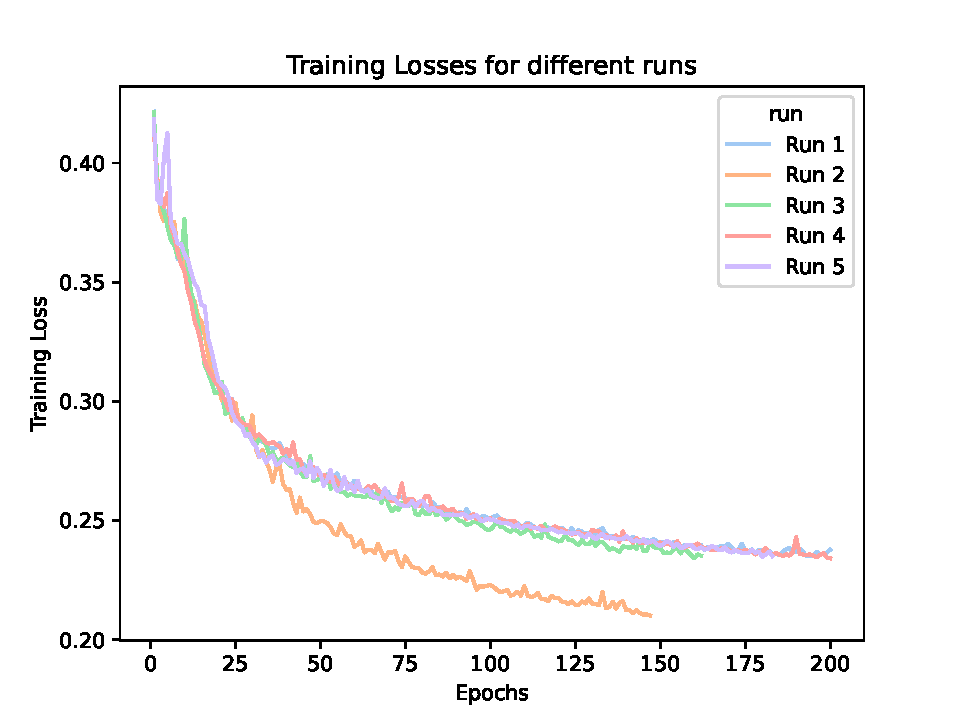
\includegraphics[width=1.0\columnwidth]{images/training_loss_diff_runs.pdf}
\caption{Training Loss on NYU Greene with different runs with the same seed. With Early Stopping and patience of 25, the 5 different runs stop their training and save the model weights at epochs 200, 147, 162, 200, 183, respectively.}
\label{fig:Training loss}
\end{figure}

\begin{figure}[htb]
\centering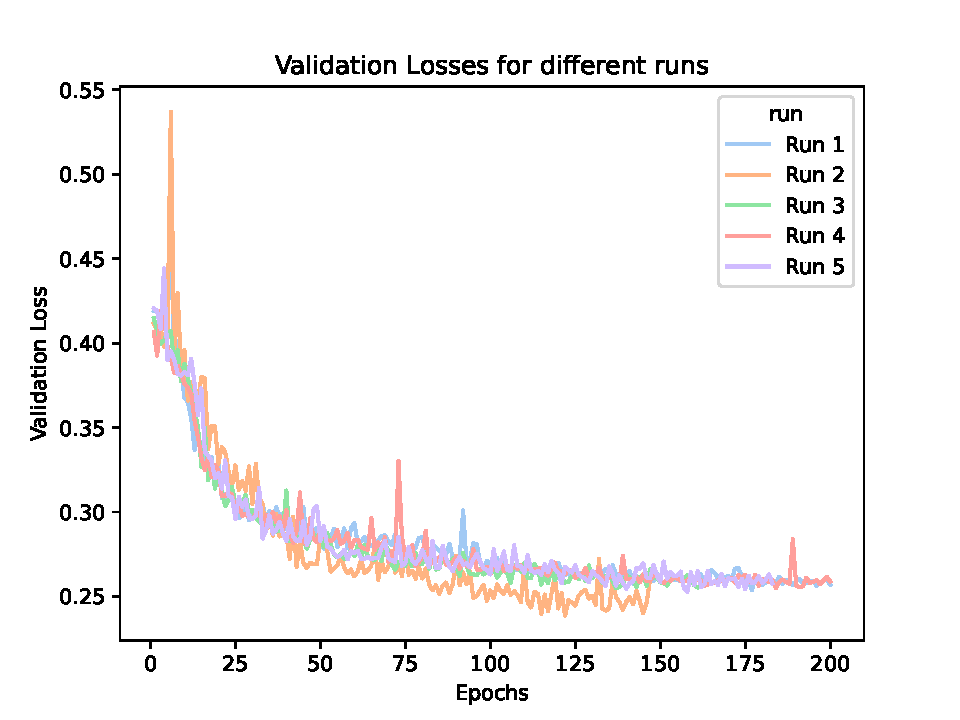
\includegraphics[width=1.0\columnwidth]{images/validation_loss_diff_runs.pdf}
\caption{Validation Loss with different runs with the same seed on on NYU Greene.}
\label{fig:Validation loss}
\end{figure}

\begin{figure}[htb]
\centering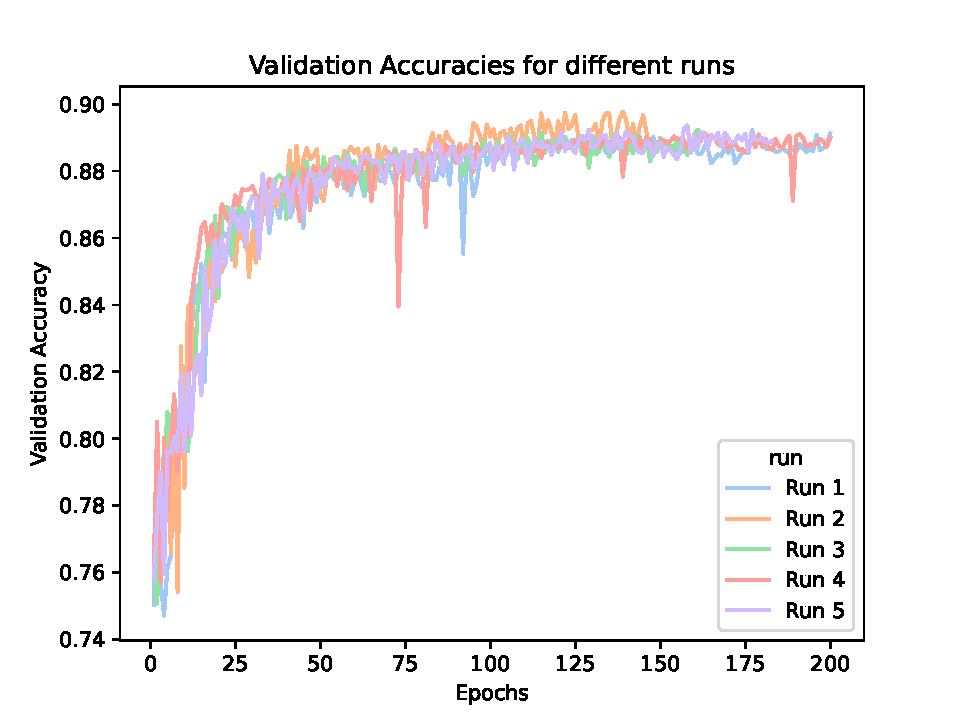
\includegraphics[width=1.0\columnwidth]{images/validation_accuracy_diff_runs.pdf}
\caption{Validation Accuracy with different runs with the same seed on NYU Greene.}
\label{fig:Validation Accuracy}
\end{figure}

\begin{figure}[htb]
\centering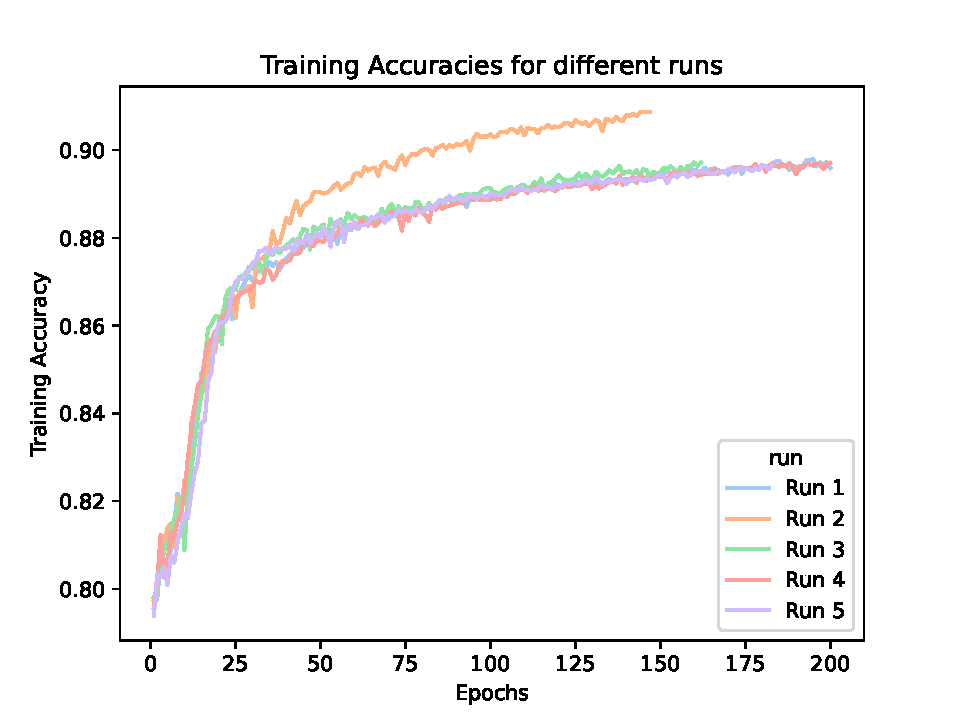
\includegraphics[width=1.0\columnwidth]{images/training_accuracy_diff_runs.pdf}
\caption{Training Accuracy with different runs with the same seed on NYU Greene.}
\label{fig:Training Accuracy}
\end{figure}

\begin{figure}[ht]
\centering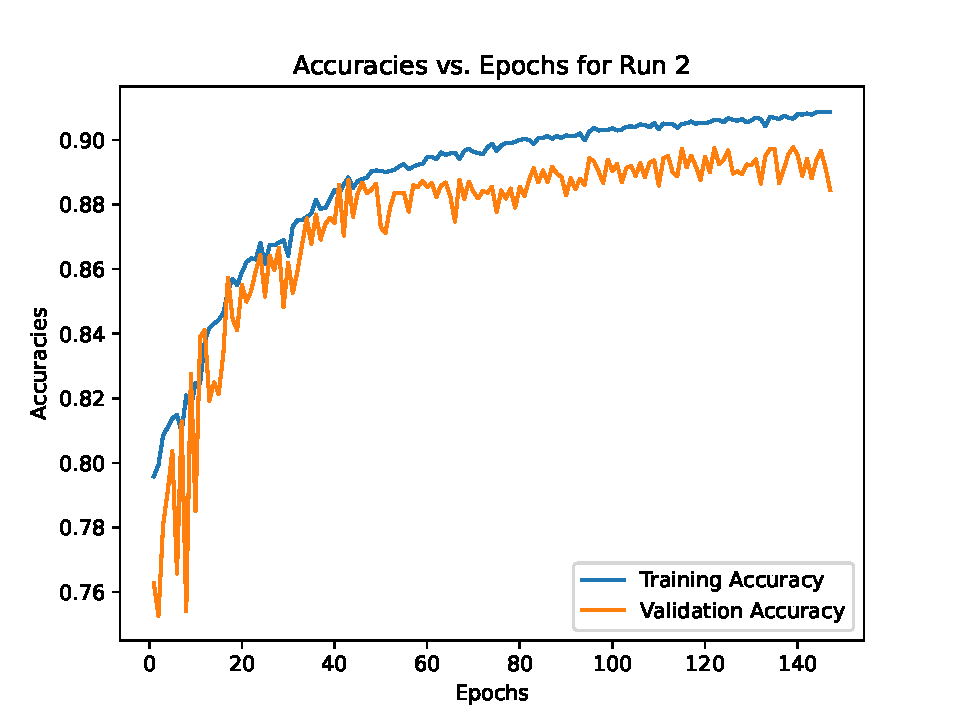
\includegraphics[width=1.0\columnwidth]{images/epoch_vs_accuracy-2.pdf}
\caption{Training and Validation Accuracy of Run 2 on NYU Greene.}
\label{fig:Accuracies of Run 2}
\end{figure}



\begin{figure}[ht]
\centering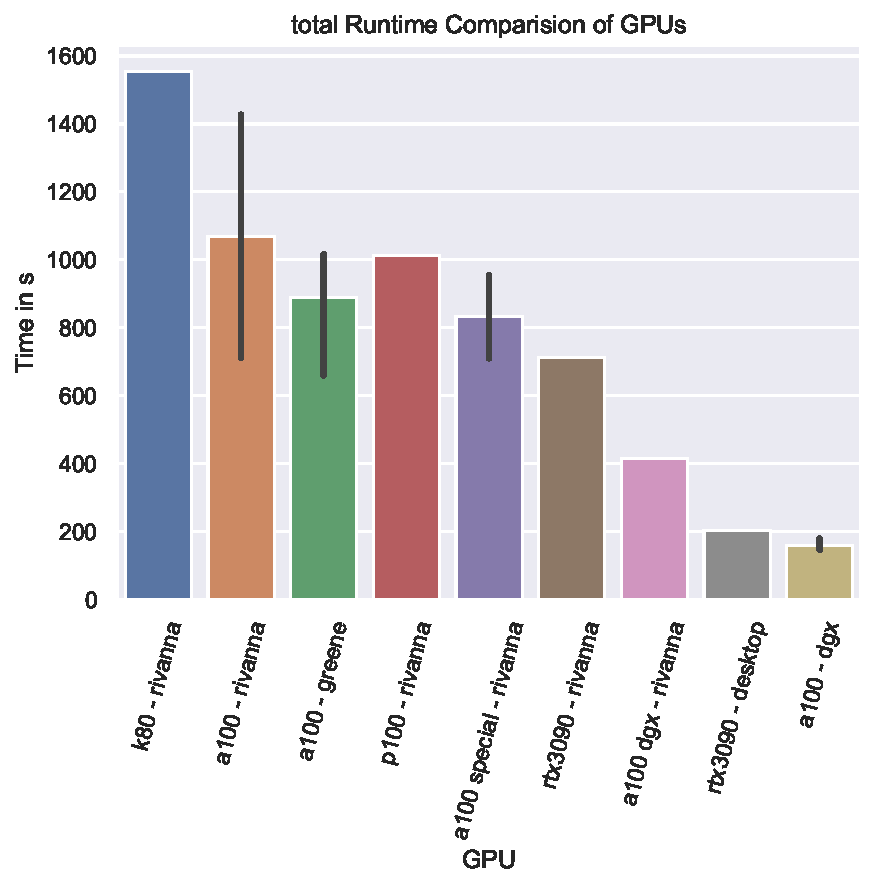
\includegraphics[width=1.0\columnwidth]{images/gregor-epoch-1.pdf}
\caption{Comparison of runtimes of cloud masking for 1 epoch on various GPUs on Rivanna, Greene, a dgx-station (a100-dgx), and the desktop \cite{las-2023-escience-cloudmask}.}
\label{fig:epoch-compare}
\end{figure}


\paragraph{Random seed on HPC systems} During the process of benchmarking we analyzed the initialization of the random number generators. Given the same seed for all runs that controls random numbers, we notice a variation of results in the different experiments. It is important to note that this is a documented feature when using GPUs and that a defined seed does not lead to number reproducibility. To be extra careful we have provided additional seed initializations for various Python libraries as documented in an earlier section.

\section{Conclusion}

In this paper, we describe our submission to MLCommons Science Cloud Masking Benchmark on two HPC systems: NYU Greene and UVA Rivanna. We also discuss, in particular, the differences between NYU and UVA team approaches in producing their benchmark results. We provide documented instructions on how to run the reference implementation on both systems for this benchmark.\footnote{Disclaimer: the documentation from NYU no longer works due to a system upgrade at NYU. A transition to Singularity from the NYU system staff was recommended. This has been independently worked on by Ruochen Gu. However, as the accounts on Greene expired, this work could not be completed and is therefore not documented in this paper. For the availability of portable code please contact G. von Laszewski.} 
The NYU team contributed a modification to the code that integrates early stopping. In addition, the NYU team developed a bash script that replicates some features provided by cloudmesh-ee while the team explored the use of SLURMs job arrays feature. We report the best scientific metric obtained on NYU's HPC and the average time taken for an epoch for training and inference on a variety of machines. The code is available in the MLCommons Science Benchmark's GitHub repository.


% conlusion can not have refernces with all the artifacts mentioned in Section \ref{sec:exp}.

\begin{acks}

  Work was in part funded by (a) NIST 60NANB21D151T (b) NSF
  CyberTraining: CIC: CyberTraining for Students and Technologies from
  Generation Z with the award numbers 1829704 and 2200409, and (c)
  Department of Energy under the grant Award No. DE-SC0023452 (d) NSF
  Collaborative Research: Framework: Software: CINES: A Scalable
  Cyberinfrastructure for Sustained Innovation in Network Engineering
  and Science with the award number 2210266. The work from the UVA
  team was conducted at the Biocomplexity Institute at
  the University of Virginia.  We like to thank the NYU AIFSR team for
  their contributions. We especially like to thank Ruochen Gu who
  continued to work on this project on a voluntary basis.


\end{acks}

%%
%% The next two lines define the bibliography style to be used, and
%% the bibliography file.
\bibliographystyle{ACM-Reference-Format}
\bibliography{vonLaszewski-cloudmask-related}

%%
%% If your work has an appendix, this is the place to put it.


\section*{Contributions}

The NYU team worked under AI for Scientific Research, a VIP group at NYU, where the team was composed of a coordinator {\em LM}, machine learning developer {\em VC}, and a researcher {\em RG}. The team was under the technical and academic supervision of {\em SS}. {\em VC} was the team’s machine learning developer who worked on setting up and experimenting on NYU’s HPC Greene with the support of UVA, as well as developing the add-on of early stopping. {\em RG} was the researcher of the group and was responsible for research in the area of cloud masking and AI benchmarking and bringing domain expertise to the group. {\em LM}  worked as the coordinator of the NYU group and was responsible for managing tasks and priorities of the project. All members of the team contributed to the code and the paper.

{\em GvL} was the technical lead at UVA and contributed the cloudmesh-ee workflow code, the cloudmesh StopWatch (which is part of cloudmesh-common), and integrated the cloudmesh timers into the code. He ran all benchmarks on Rivanna and the Desktop.  He facilitates the submission to MLCommons. {\em GvL}, {\em GCF}, and {\em JP} provided general direction for the project including feedback on the progress of code development as well as benchmarking. {\em GvL} contributed to code development by the NYU team, the paper, and facilitated many hackathons with the NYU team. {\em SJ} and {\em JP} provided the original cloud masking implementation and developed the new accuracy value to which {\em GvL} contributed. For UVA {\em GvL} also developed workflow-related code to integrate VPN authentication, GPU energy monitoring, the initial documentation to port the code on other machines, and the development of a reusable Singularity container for the application. Through using cloudmesh-ee a portable code using the FAIR principle is available by UVA.

\end{document}
\endinput
%%
%% End of file `sample-sigplan.tex'.

